
\documentclass[10pt,a4paper]{article}
\usepackage{f1000_styles}

%% Default: numerical citations
% \usepackage[numbers]{natbib}

%% Uncomment this lines for superscript citations instead
% \usepackage[super]{natbib}

%% Uncomment these lines for author-year citations instead
% \usepackage[round]{natbib}
% \let\cite\citep

%% lines required to use a CSL style for references
\newlength{\cslhangindent}
\setlength{\cslhangindent}{1.5em}
\newlength{\csllabelwidth}
\setlength{\csllabelwidth}{3em}
\newlength{\cslentryspacingunit} % times entry-spacing
\setlength{\cslentryspacingunit}{\parskip}
\newenvironment{CSLReferences}[2] % #1 hanging-ident, #2 entry spacing
 {% don't indent paragraphs
  \setlength{\parindent}{0pt}
  % turn on hanging indent if param 1 is 1
  \ifodd #1
  \let\oldpar\par
  \def\par{\hangindent=\cslhangindent\oldpar}
  \fi
  % set entry spacing
  \setlength{\parskip}{#2\cslentryspacingunit}
 }%
 {}
\usepackage{calc}
\newcommand{\CSLBlock}[1]{#1\hfill\break}
\newcommand{\CSLLeftMargin}[1]{\parbox[t]{\csllabelwidth}{#1}}
\newcommand{\CSLRightInline}[1]{\parbox[t]{\linewidth - \csllabelwidth}{#1}\break}
\newcommand{\CSLIndent}[1]{\hspace{\cslhangindent}#1}

%% lines to get the code chunks working

%% lines to enable bulletpoints in a new notation style
\providecommand{\tightlist}{%
  \setlength{\itemsep}{0pt}\setlength{\parskip}{0pt}}

\begin{document}
\pagestyle{fancy}

\title{Applying a Multiverse to Habitat Analyses}
\author[1]{Benjamin Michael Marshall*}
\author[1]{Alexander Bradley Duthie**}
\affil[1]{Biological and Environmental Sciences, Faculty of Natural Sciences, University of Stirling, Stirling, FK9 4LA, Scotland, UK}

\affil[*]{\href{mailto:benjaminmichaelmarshall@gmail.com}{\nolinkurl{benjaminmichaelmarshall@gmail.com}}}
\affil[**]{\href{mailto:alexander.duthie@stir.ac.uk}{\nolinkurl{alexander.duthie@stir.ac.uk}}}

\maketitle
\thispagestyle{fancy}

\begin{abstract}

---

\end{abstract}

\section*{Keywords}

Movement ecology, simulation

\clearpage
\pagestyle{fancy}

\hypertarget{multiverse-introduction}{%
\section{Multiverse Introduction}\label{multiverse-introduction}}

\hypertarget{research-flexibilty-and-the-justification-for-a-multiverse-approach}{%
\subsection{Research flexibilty and the justification for a multiverse approach}\label{research-flexibilty-and-the-justification-for-a-multiverse-approach}}

Researchers are intrinsically part of the research process (\protect\hyperlink{ref-levins_dialectical_1985}{Levins \& Lewontin, 1985}; \protect\hyperlink{ref-tang-martinez_history_2020}{Tang-Martínez, 2020}), and our expectations can shape the answers we find (\protect\hyperlink{ref-holman_evidence_2015}{Holman et al., 2015}).
While we can strive to conduct research objectively, there are frequent moments during research that require judgement calls (\protect\hyperlink{ref-steegen_increasing_2016}{Steegen et al., 2016}).
Such calls, choices, or decisions occur throughout the research process, encompassing everything from study design (e.g., sample size, sampling intensity, sample stratification) to analysis (e.g., Bayesian or frequentist, ex/inclusion of outliers).
We draw on our own experience and the input of peers to try and ensure the best choices are made to produce robust and reliable results, but we also contend with data, expertise, and interpretability constraints (\protect\hyperlink{ref-liu_paths_2020}{Liu, Althoff \& Heer, 2020}).

Researchers are also influenced by the incentive system around them (\protect\hyperlink{ref-anderson_perverse_2007}{Anderson et al., 2007}).
We cannot undertake research in a vacuum; we often require institutions, funders, and scientific journals to produce and share research.
These bodies can influence what research is conducted; they are in a position to incentivise or disincentivise research of certain topics or methodologies (\protect\hyperlink{ref-fanelli_pressures_2010}{Fanelli, 2010a}; \protect\hyperlink{ref-ware_significance_2015}{Ware \& Munafò, 2015}; \protect\hyperlink{ref-smaldino_natural_2016}{Smaldino \& McElreath, 2016}).
The use of impact factor (and other similar metrics) is an example of citations being used as a measure of quality or research worth.
But when examined closer, the impact factor appears detached from the robustness or reliability of the research (\protect\hyperlink{ref-Brembs2018}{Brembs, 2018}).
This decrease in robustness can be seen in the increases in effect sizes inflation, p-value misreporting, among a number of other measures of quality (\protect\hyperlink{ref-Brembs2018}{Brembs, 2018}).
Similarly, novelty has been fetishised by journals to the detriment of replications studies (\protect\hyperlink{ref-vinkers_use_2015}{Vinkers, Tijdink \& Otte, 2015}; \protect\hyperlink{ref-forstmeier_detecting_2017}{Forstmeier, Wagenmakers \& Parker, 2017}; \protect\hyperlink{ref-brembs_reliable_2019}{Brembs, 2019}), despite widespread agreement on the importance of replications (\protect\hyperlink{ref-fraser_role_2020}{Fraser et al., 2020}).
There is a bias towards positive, statistically significant results (\protect\hyperlink{ref-jennions_publication_2002}{Jennions \& Møller, 2002}; \protect\hyperlink{ref-cassey_survey_2004}{Cassey et al., 2004}).
Due to the nature of frequentist statistical significance, a prioritisation of significant results can elevate underpowered studies and boost false positive rates (\protect\hyperlink{ref-forstmeier_cryptic_2011}{Forstmeier \& Schielzeth, 2011}; \protect\hyperlink{ref-albers_problem_2019}{Albers, 2019}).

Unfortunately, there is evidence that the system of incentives trickle down to impact the judgement calls and decisions of researchers while undertaking research and when publishing those results.
The more detrimental of these decisions have been termed questionable research practices (\protect\hyperlink{ref-fraser_questionable_2018}{Fraser et al., 2018}; \protect\hyperlink{ref-bishop_rein_2019}{Bishop, 2019}).
They chiefly come in three forms: HARKing, cherry-picking, and p-hacking.
Hypothesising After Results Known (HARKing) is where the research can present the results as a confirmatory result, despite originally there being no or contrary hypothesis.
HARKing can sometimes be further enabled and rationalised by hindsight bias, where unexpected results are perceived as more likely once they have been observed (\protect\hyperlink{ref-gelman_garden_2013}{Gelman \& Loken, 2013}; \protect\hyperlink{ref-forstmeier_detecting_2017}{Forstmeier, Wagenmakers \& Parker, 2017}).
Cherry-picking is the removal or non-reporting of data points or (co-)variables, that did not yield significant results.
P-hacking is the repeated use of statistical tests, with different settings, to achieve statistical significance.
Arguably, the existence of p-hacking is enabled by an over-reliance on p-value thresholds, rather than flexible p-value thresholds that are predefined based on effect size of interest, sample size, and desired accuracy of estimation (\protect\hyperlink{ref-lakens_justify_2018}{Lakens et al., 2018}).
Questionable research practices can be viewed as methods to achieve a neat, statistically significant, and publishable narrative (\protect\hyperlink{ref-oboyle_chrysalis_2014}{O'Boyle, Banks \& Gonzalez-Mulé, 2014}); in the worse cases, narratives could be prioritised over transparently reported results.

There is a fear that questionable research practices, and the broader incentives they are connected to, are responsible for the replicability crisis (often referred to as the ``reproducibility crisis''). Across many disciplines, there are examples of replication studies being unable to replicate prior research (\protect\hyperlink{ref-freedman_economics_2015}{Freedman, Cockburn \& Simcoe, 2015}; \protect\hyperlink{ref-open_science_collaboration_estimating_2015}{Open Science Collaboration, 2015}; \protect\hyperlink{ref-kelly_rate_2019}{Kelly, 2019}).
Often these replication efforts are conducted with larger sample sizes, or rely on the consolidation of many independent studies (often in the form of meta-analyses).
The implication is not that the original studies were necessarily flawed; but -- in the absence of questionable research practices -- sufficient variation exists in the study subjects to obscure a consistent effect {[}i.e., variation beyond variation stemming from sampling; Simonsohn (\protect\hyperlink{ref-simonsohn_small_2015}{2015}){]}.

However, variation can also stem from analysis flexibility (i.e., the presence of many ways to analyse the same data to answer the same question).
This flexibility helps enable questionable research practices (\protect\hyperlink{ref-fraser_questionable_2018}{Fraser et al., 2018}), and is potentially steered by publication bias (\protect\hyperlink{ref-jennions_publication_2002}{Jennions \& Møller, 2002}; \protect\hyperlink{ref-cassey_survey_2004}{Cassey et al., 2004}) if results that produce more publishable results are prioritised/rewarded over less exciting but robust results.
Given the prominence of questionable research practices and publication bias, the inconsistencies between initial and replication studies warrant investigation (especially when analysis flexibility is also implicated in potentially flawed replications \protect\hyperlink{ref-bryan_replicator_2019}{Bryan, Yeager \& O'Brien, 2019}).
It is key to note that analysis flexibility can still lead to variable results in the absence of any undesirable incentives simply as the result of researchers considering different approaches of differing validities for a given dataset (\protect\hyperlink{ref-gelman_garden_2013}{Gelman \& Loken, 2013}).

Scientific progress requires building upon past results, and therefore requires confidence in past results.
Issues arise when subsequent research is based upon weak foundations --i.e., studies with a limited capacity to be replicated because of questionable practices or over-generalisation.
Early significant results can dictate the direction of research and grow resistant to later contradictory results (\protect\hyperlink{ref-barto_dissemination_2012}{Barto \& Rillig, 2012}); therefore, early diagnoses of overly confident results or previously unknown sources of variation becomes a priority.

In medical fields, a lack of replicability comes with direct monetary and well-being costs (\protect\hyperlink{ref-freedman_economics_2015}{Freedman, Cockburn \& Simcoe, 2015}).
Like the medical field, ecological studies can come with well-being costs to the study subjects {[}e.g., direct surgery/marking of the animal (\protect\hyperlink{ref-Reinert1982}{Reinert \& Cundall, 1982}; \protect\hyperlink{ref-Winne2006}{Winne et al., 2006}){]}, as well as impacts on stakeholders stemming from management decisions.
There are fears that the lack of replicability will feed distrust of science more generally (\protect\hyperlink{ref-anvari_replicability_2018}{Anvari \& Lakens, 2018}).
Therefore, maximising replicability in ecology is key to minimising research waste (\protect\hyperlink{ref-grainger_evidence_2019}{Grainger et al., 2019}) and the negative impacts on systems and subjects studied.

The impacts on the study subjects, paired with the often high monetary costs of ecological studies (particularly bio-logging where animals may undergo surgery, \protect\hyperlink{ref-weaver_technology_2021}{Weaver, Westphal \& Taylor, 2021}) means that replications can be more difficult to justify.
When paired with fact that ecological systems are complex and in constant flux --often frustrating perfect replications due to changes in space and time (\protect\hyperlink{ref-nakagawa_replicating_2015}{Nakagawa \& Parker, 2015}; \protect\hyperlink{ref-schnitzer_would_2016}{Schnitzer \& Carson, 2016}) --we are left with a distinct lack of direct replications in ecology (\protect\hyperlink{ref-kelly_rate_2019}{Kelly, 2019}).

The low prevalence of replications in ecology make it difficult to assess the overall irreplicabilty situation in ecology (\protect\hyperlink{ref-kelly_rate_2019}{Kelly, 2019}); but there are several examples that suggest irreplicabilty is something ecologists should be wary of (\protect\hyperlink{ref-wang_irreproducible_2018}{Wang et al., 2018}; \protect\hyperlink{ref-sanchez-tojar_meta-analysis_2018}{Sánchez-Tójar et al., 2018}; \protect\hyperlink{ref-roche_behavioural_2020}{Roche et al., 2020}; \protect\hyperlink{ref-clark_ocean_2020}{Clark et al., 2020}).
The potential for irreplicabilty is further supported by evidence of positive publication bias (\protect\hyperlink{ref-fanelli_positive_2010}{Fanelli, 2010b}, \protect\hyperlink{ref-fanelli_negative_2012}{2012}), and links between smaller sample sizes and inflated effect sizes (\protect\hyperlink{ref-lemoine_underappreciated_2016}{Lemoine et al., 2016}).

In the absence of direct replications, ecology is often left to assess replicability via conceptual replications (\protect\hyperlink{ref-fraser_role_2020}{Fraser et al., 2020}) or efforts broadly referred to as quasi-replications (\protect\hyperlink{ref-palmer_quasi-replication_2000}{Palmer, 2000}).
Replications range in intensity. Direct (or exact) replications are attempts to replicate a tightly defined concept/hypothesis while duplicating of all characteristics of the original study.
Partial replications are a step looser, where the concept/hypothesis tested is less clearly defined (e.g., applicable to a broader scale) but efforts are made to repeat the same methodology.
The most general category are conceptual replications, where the subject and method of study varies from the original study, but the replication targets a the same concept/hypothesis (\protect\hyperlink{ref-nakagawa_replicating_2015}{Nakagawa \& Parker, 2015}; \protect\hyperlink{ref-kelly_rate_2019}{Kelly, 2019}).
Both partial and conceptual can be classed as quasi-replications if the concept and scale is broadly defined (\protect\hyperlink{ref-nakagawa_replicating_2015}{Nakagawa \& Parker, 2015}).

Conceptual replications are extremely valuable, but rely on our ability to compare replication efforts to previous findings.
An important aspect of those comparisons is accounting for factors differing between the studies that are not salient to the effect of interest (\protect\hyperlink{ref-forstmeier_detecting_2017}{Forstmeier, Wagenmakers \& Parker, 2017}); e.g., those linked to sampling differences (\protect\hyperlink{ref-simonsohn_small_2015}{Simonsohn, 2015}).
An example of sampling differences leading to differences in final results can be seen in the case of reptile space use.
Silva et al. (\protect\hyperlink{ref-silva_reptiles_2020}{2020}) showed how frequently a reptile was located by a researcher interacted with the space-use estimation method, leading to large differences in area estimates even when using the same estimation method.
What is revealing is not only how the choices during analysis (e.g., choice of area estimation method) impacted results, but how the error introduced by those choices changed depending on the sampling.
It presents a scenario where the \emph{correct} choice was dependent on preceding decisions when designing the study; therefore, highlighting the need to explore the impacts of multiple decisions simultaneously.

As seen in the reptile space use example, the choices made by the researcher {[}researcher degrees of freedom; Simmons, Nelson \& Simonsohn (\protect\hyperlink{ref-simmons_false-positive_2011}{2011}){]} is a key source of variation among studies.
It would be advantageous to understand which choices have a significant impact and whether we can account for differences in choice during comparisons.
An understanding of choice could better guide decisions during a study and potentially be used to gauge the robustness of a given dataset in answering a given question.

Research degrees of freedom {[}or flexibility in analysis; Forstmeier, Wagenmakers \& Parker (\protect\hyperlink{ref-forstmeier_detecting_2017}{2017}){]} have been elegantly demonstrated by a number of ``many analysts'' studies (e.g., \protect\hyperlink{ref-silberzahn_many_2018}{Silberzahn et al., 2018}; \protect\hyperlink{ref-huntingtonklein_influence_2021}{Huntington‐Klein et al., 2021}).
In these studies, a number of researchers, or research groups, are tasked with answering the same question.
Naturally each participant takes a slightly different approach, both in how the question is interpreted (\protect\hyperlink{ref-auspurg_has_2021}{Auspurg \& Brüderl, 2021}), and the analysis approach chosen (\protect\hyperlink{ref-gelman_garden_2013}{Gelman \& Loken, 2013}; \protect\hyperlink{ref-bastiaansen_time_2020}{Bastiaansen et al., 2020}), resulting is different final results.
The variation in final results can be considered originating from six sources of uncertainty/variation (\protect\hyperlink{ref-hoffmann_multiplicity_2021}{Hoffmann et al., 2021}): measurement (randomness from the act of measuring), data preprocessing (decisions on data inclusion/exclusion and transforming), parameter (decisions on which parameters used as covariates/predictors), model (decisions on model structure and specification), method (decisions on method choice and parameterisation), and sampling (randomness as a result of sampling a wider population).
Several sources of variation (data preprocessing, parameter, model, and method) are likely to be particularly key to defining researcher degrees of freedom post data collection.
In some cases, the cause behind the variability in results is hard to diagnose (\protect\hyperlink{ref-breznau_observing_2021}{Breznau et al., 2021}), or will be less likely to be questioned because of the agreement with existing theory (\protect\hyperlink{ref-gelman_garden_2013}{Gelman \& Loken, 2013}).
There are examples where the variation in results is sufficient to change the final conclusions (\protect\hyperlink{ref-salis_how_2021}{Salis, Lena \& Lengagne, 2021}), and others where it alters the strength of an estimated effect (\protect\hyperlink{ref-desbureaux_subjective_2021}{Desbureaux, 2021}).
The importance of the effect size variation is context specific, i.e., how variation relates to the overall effect size, and can impact results pertaining to real-world scenarios (\protect\hyperlink{ref-desbureaux_subjective_2021}{Desbureaux, 2021}).

\hypertarget{multiverse-analysis}{%
\subsection{Multiverse analysis}\label{multiverse-analysis}}

A rising approach to address the unknown impacts of undisclosed researcher degrees of freedom is to fully explore all plausible or reasonable analysis choices open to researchers -- to explore a multiverse of design choices (\protect\hyperlink{ref-steegen_increasing_2016}{Steegen et al., 2016}).
This multiverse analysis -- closely linked to vibration of effects (\protect\hyperlink{ref-patel_assessment_2015}{Patel, Burford \& Ioannidis, 2015}), multi-model analysis (\protect\hyperlink{ref-young_model_2017}{Young \& Holsteen, 2017}), and specification curve analysis (\protect\hyperlink{ref-simonsohn_specification_2020}{Simonsohn, Simmons \& Nelson, 2020})-- has the potential to demonstrate and quantify the variation stemming from researcher's analyses choices (\protect\hyperlink{ref-rijnhart_assessing_2021}{Rijnhart et al., 2021}).
Choices can include everything from from sample sizes and splits (e.g., \protect\hyperlink{ref-webb_multiverse_2021}{Webb \& Demeyere, 2021}) to measurement and summary statistics (e.g., \protect\hyperlink{ref-parsons_exploring_2020}{Parsons, 2020}), but crucially should only include options that are reasonable (\protect\hyperlink{ref-simonsohn_specification_2020}{Simonsohn, Simmons \& Nelson, 2020}; \protect\hyperlink{ref-del_giudice_travelers_2021}{Del Giudice \& Gangestad, 2021}).
What counts as reasonable is not necessarily simple, and inclusion of irrelevant choices can easily mask important choices because of the multiplicative nature of a branching path network (\protect\hyperlink{ref-del_giudice_travelers_2021}{Del Giudice \& Gangestad, 2021}) (Fig. \ref{fig:multiDiagram}).
Construction of a multiverse requires justification of which decisions are treated as variable, and why there is not an \emph{a priori} and defensible single solution (\protect\hyperlink{ref-del_giudice_travelers_2021}{Del Giudice \& Gangestad, 2021}).
A multiverse populated with well-justified decisions allows the exploration of which choices inflate variation between analysis universes, while also offering insights into how to deflate variation {[}e.g., refinement of initial study design, the removal of ambiguities like tightening categories definitions; Steegen et al. (\protect\hyperlink{ref-steegen_increasing_2016}{2016}){]}.

\begin{figure}
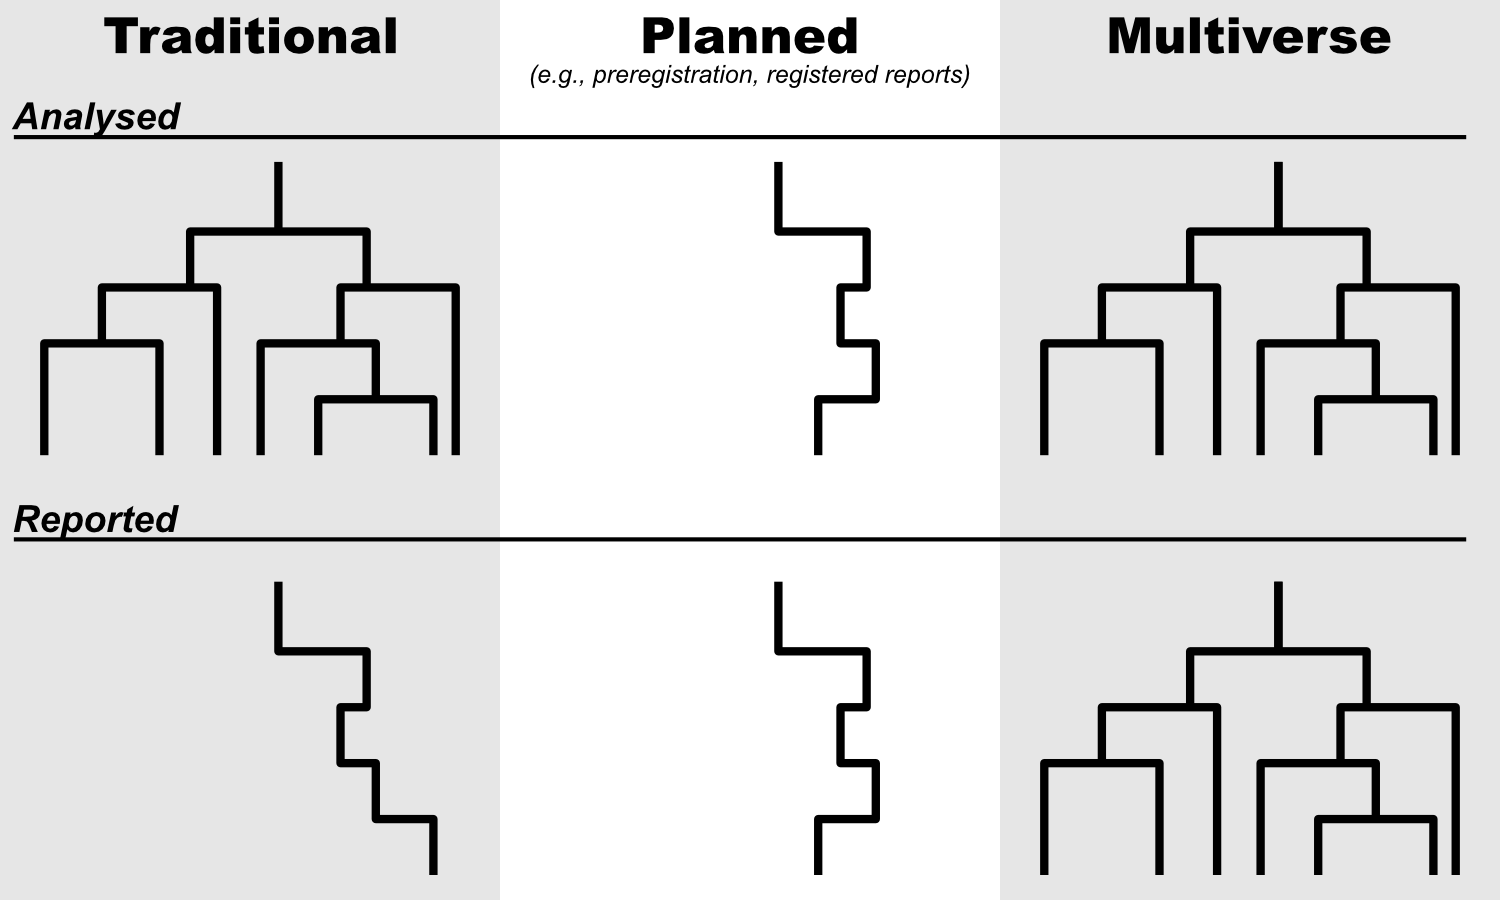
\includegraphics[width=1\linewidth]{../ext_images/Multiverse compared diagram} \caption{Diagram showing how multiverse analysis differs from other approaches. Each branch node represents a choice made during aysnalis}\label{fig:multiDiagram}
\end{figure}

Ecological systems are complex to study and frustrate replication efforts (\protect\hyperlink{ref-nakagawa_replicating_2015}{Nakagawa \& Parker, 2015}; \protect\hyperlink{ref-schnitzer_would_2016}{Schnitzer \& Carson, 2016}), and in the case of movement ecology, the data analysed (i.e., derived data, such as step length, speed, and turn angle derived from timestamped coordinate data) require multiple stages of preprocessing.
Therefore, multiverse analysis is an avenue to explore causes of variation between studies without the additional costs of practical studies, while also being capable of exploring data processing decisions that may not have immediately apparent impacts on final results.

If the data entropy (the process in which as data ages the chances of irreversible loss increase, \protect\hyperlink{ref-vines_availability_2014}{Vines et al., 2014}) and resistance to data sharing (\protect\hyperlink{ref-miyakawa_no_2020}{Miyakawa, 2020}; \protect\hyperlink{ref-tedersoo_data_2021}{Tedersoo et al., 2021}) can be overcome, we will be able to retroactively explore the impact of researcher degrees of freedom on ecological studies (\protect\hyperlink{ref-rijnhart_assessing_2021}{Rijnhart et al., 2021}).
Such retroactive assessment is an attractive option when other methods to explore false positive rates (\protect\hyperlink{ref-hoffmann_multiplicity_2021}{Hoffmann et al., 2021}), such as preregistration and registered reports (\protect\hyperlink{ref-kaplan_likelihood_2015}{Kaplan \& Irvin, 2015}; \protect\hyperlink{ref-scheel_excess_2021}{Scheel, Schijen \& Lakens, 2021}), will require more time to yield results.
Ideally we can use multiverse analysis with preregistrations to boost transparency surrounding the inclusion of decisions and the rationale behind others exclusions (\protect\hyperlink{ref-dragicevic_increasing_2019}{Dragicevic et al., 2019}; \protect\hyperlink{ref-simonsohn_specification_2020}{Simonsohn, Simmons \& Nelson, 2020}).
Given the success of meta-analyses to overcome short-comings in the publication record {[}e.g., p-hacking; Head et al. (\protect\hyperlink{ref-head_extent_2015}{2015}){]}, multiverse analysis may aid the direction of future research efforts by providing a means of meeting calls to replicate results before collecting more (\protect\hyperlink{ref-nuijten_verify_2018}{Nuijten et al., 2018}).

However, as not all choices are equally valid, so multiverse analysis cannot simply provide a correct answer (\protect\hyperlink{ref-steegen_increasing_2016}{Steegen et al., 2016}) --the ``average'' result is not necessarily the closest to the truth.
If we were to undertake a multiverse analysis in a scenario with a ``known truth'', i.e., using a simulated dataset (\protect\hyperlink{ref-bastiaansen_time_2020}{Bastiaansen et al., 2020}), we may be able to detect identify the amount of variation from different sources {[}e.g, biological variation vs study design variation; Breznau et al. (\protect\hyperlink{ref-breznau_observing_2021}{2021}){]}, and potentially the systematic biases stemming from specific choices (potentially via Bayesian Casual Forests \protect\hyperlink{ref-bryan_replicator_2019}{Bryan, Yeager \& O'Brien, 2019}).

Use of simulated data is an established way to explore the robustness of methodologies (\protect\hyperlink{ref-minchin_simulation_1987}{Minchin, 1987}; \protect\hyperlink{ref-silva_reptiles_2020}{Silva et al., 2020}); and this project will harness the benefits of simulated data to assess the impacts of researcher degrees of freedom on the results garnered from animal movement datasets via a multiverse approach.
The initial step will be to develop an animal movement simulation where we can input an often of-interest parameter (e.g., preference for a particular habitat type).
The goal of the multiverse will be to run a multitude of sampling/data processing/analysis approaches on that simulated animal movement data, to determine which pathway or series of decisions gets closest to the predefined parameter used to simulate the data initially.
If a sufficiently diverse set of scenarios can be explored in the multiverse, the third step will be applying the now know uncertainty from particular choices to explore whether different choices would have changed conclusions in real-world datasets.

\hypertarget{references}{%
\section*{References}\label{references}}
\addcontentsline{toc}{section}{References}

\hypertarget{refs}{}
\begin{CSLReferences}{1}{0}
\leavevmode\vadjust pre{\hypertarget{ref-albers_problem_2019}{}}%
Albers C. 2019. The problem with unadjusted multiple and sequential statistical testing. \emph{Nature Communications} 10:1921. DOI: \href{https://doi.org/10.1038/s41467-019-09941-0}{10.1038/s41467-019-09941-0}.

\leavevmode\vadjust pre{\hypertarget{ref-anderson_perverse_2007}{}}%
Anderson MS, Ronning EA, De Vries R, Martinson BC. 2007. The {Perverse} {Effects} of {Competition} on {Scientists}' {Work} and {Relationships}. \emph{Science and Engineering Ethics} 13:437--461. DOI: \href{https://doi.org/10.1007/s11948-007-9042-5}{10.1007/s11948-007-9042-5}.

\leavevmode\vadjust pre{\hypertarget{ref-anvari_replicability_2018}{}}%
Anvari F, Lakens D. 2018. The replicability crisis and public trust in psychological science. \emph{Comprehensive Results in Social Psychology} 3:266--286. DOI: \href{https://doi.org/10.1080/23743603.2019.1684822}{10.1080/23743603.2019.1684822}.

\leavevmode\vadjust pre{\hypertarget{ref-auspurg_has_2021}{}}%
Auspurg K, Brüderl J. 2021. Has the {Credibility} of the {Social} {Sciences} {Been} {Credibly} {Destroyed}? {Reanalyzing} the {``{Many} {Analysts}, {One} {Data} {Set}''} {Project}. \emph{Socius: Sociological Research for a Dynamic World} 7:237802312110244. DOI: \href{https://doi.org/10.1177/23780231211024421}{10.1177/23780231211024421}.

\leavevmode\vadjust pre{\hypertarget{ref-barto_dissemination_2012}{}}%
Barto EK, Rillig MC. 2012. Dissemination biases in ecology: Effect sizes matter more than quality. \emph{Oikos} 121:228--235. DOI: \href{https://doi.org/10.1111/j.1600-0706.2011.19401.x}{10.1111/j.1600-0706.2011.19401.x}.

\leavevmode\vadjust pre{\hypertarget{ref-bastiaansen_time_2020}{}}%
Bastiaansen JA, Kunkels YK, Blaauw FJ, Boker SM, Ceulemans E, Chen M, Chow S-M, Jonge P de, Emerencia AC, Epskamp S, Fisher AJ, Hamaker EL, Kuppens P, Lutz W, Meyer MJ, Moulder R, Oravecz Z, Riese H, Rubel J, Ryan O, Servaas MN, Sjobeck G, Snippe E, Trull TJ, Tschacher W, Veen DC van der, Wichers M, Wood PK, Woods WC, Wright AGC, Albers CJ, Bringmann LF. 2020. Time to get personal? {The} impact of researchers choices on the selection of treatment targets using the experience sampling methodology. \emph{Journal of Psychosomatic Research} 137:110211. DOI: \href{https://doi.org/10.1016/j.jpsychores.2020.110211}{10.1016/j.jpsychores.2020.110211}.

\leavevmode\vadjust pre{\hypertarget{ref-bishop_rein_2019}{}}%
Bishop D. 2019. Rein in the four horsemen of irreproducibility. \emph{Nature} 568:435--435. DOI: \href{https://doi.org/10.1038/d41586-019-01307-2}{10.1038/d41586-019-01307-2}.

\leavevmode\vadjust pre{\hypertarget{ref-Brembs2018}{}}%
Brembs B. 2018. Prestigious {Science} {Journals} {Struggle} to {Reach} {Even} {Average} {Reliability}. \emph{Frontiers in Human Neuroscience} 12:1--7. DOI: \href{https://doi.org/10.3389/fnhum.2018.00037}{10.3389/fnhum.2018.00037}.

\leavevmode\vadjust pre{\hypertarget{ref-brembs_reliable_2019}{}}%
Brembs B. 2019. Reliable novelty: {New} should not trump true. \emph{PLOS Biology} 17:e3000117. DOI: \href{https://doi.org/10.1371/journal.pbio.3000117}{10.1371/journal.pbio.3000117}.

\leavevmode\vadjust pre{\hypertarget{ref-breznau_observing_2021}{}}%
Breznau N, Rinke EM, Wuttke A, Adem M, Adriaans J, Alvarez-Benjumea A, Andersen HK, Auer D, Azevedo F, Bahnsen O, Balzer D, Bauer G, Bauer P, Baumann M, Baute S, Benoit V, Bernauer J, Berning C, Berthold A, Bethke FS, Biegert T, Blinzler K, Blumenberg J, Bobzien L, Bohman A, Bol T, Bostic A, Brzozowska Z, Burgdorf K, Burger K, Busch K, Castillo JC, Chan N, Christmann P, Connelly R, Czymara CS, Damian E, Ecker A, Edelmann A, Eger MA, Ellerbrock S, Forke A, Forster AG, Gaasendam C, Gavras K, Gayle V, Gessler T, Gnambs T, Godefroidt A, Grömping M, Groß M, Gruber S, Gummer T, Hadjar A, Heisig JP, Hellmeier S, Heyne S, Hirsch M, Hjerm M, Hochman O, Hövermann A, Hunger S, Hunkler C, Huth N, Ignacz Z, Jacobs L, Jacobsen J, Jaeger B, Jungkunz S, Jungmann N, Kauff M, Kleinert M, Klinger J, Kolb J-P, Kołczyńska M, Kuk JS, Kunißen K, Sinatra DK, Greinert A, Lersch PM, Löbel L-M, Lutscher P, Mader M, Madia JE, Malancu N, Maldonado L, Marahrens H, Martin N, Martinez P, Mayerl J, Mayorga OJ, McManus P, Wagner K, Meeusen C, Meierrieks D, Mellon J, Merhout F, Merk S, Meyer D, Micheli L, Mijs JJB, Moya C, Neunhoeffer M, Nüst D, Nygård O, Ochsenfeld F, Otte G, Pechenkina A, Prosser C, Raes L, Ralston K, Ramos M, Roets A, Rogers J, Ropers G, Samuel R, Sand G, Schachter A, Schaeffer M, Schieferdecker D, Schlueter E, Schmidt K, Schmidt R, Schmidt-Catran A, Schmiedeberg C, Schneider J, Schoonvelde M, Schulte-Cloos J, Schumann S, Schunck R, Schupp J, Seuring J, Silber H, Sleegers WWA, Sonntag N, Staudt A, Steiber N, Steiner N, Sternberg S, Stiers D, Stojmenovska D, Storz N, Striessnig E, Stroppe A-K, Teltemann J, Tibajev A, Tung BB, Vagni G, Van Assche J, Linden M van der, Noll J van der, Van Hootegem A, Vogtenhuber S, Voicu B, Wagemans F, Wehl N, Werner H, Wiernik BM, Winter F, Wolf C, Yamada Y, Zhang N, Ziller C, Zins S, Żółtak T, Nguyen HHV. 2021. Observing {Many} {Researchers} {Using} the {Same} {Data} and {Hypothesis} {Reveals} a {Hidden} {Universe} of {Uncertainty}. \emph{MetaArXiv}. DOI: \href{https://doi.org/10.31222/osf.io/cd5j9}{10.31222/osf.io/cd5j9}.

\leavevmode\vadjust pre{\hypertarget{ref-bryan_replicator_2019}{}}%
Bryan CJ, Yeager DS, O'Brien JM. 2019. Replicator degrees of freedom allow publication of misleading failures to replicate. \emph{Proceedings of the National Academy of Sciences} 116:25535--25545. DOI: \href{https://doi.org/10.1073/pnas.1910951116}{10.1073/pnas.1910951116}.

\leavevmode\vadjust pre{\hypertarget{ref-cassey_survey_2004}{}}%
Cassey P, Ewen JG, Blackburn TM, Møller AP. 2004. A survey of publication bias within evolutionary ecology. \emph{Proceedings of the Royal Society of London. Series B: Biological Sciences} 271. DOI: \href{https://doi.org/10.1098/rsbl.2004.0218}{10.1098/rsbl.2004.0218}.

\leavevmode\vadjust pre{\hypertarget{ref-clark_ocean_2020}{}}%
Clark TD, Raby GD, Roche DG, Binning SA, Speers-Roesch B, Jutfelt F, Sundin J. 2020. Ocean acidification does not impair the behaviour of coral reef fishes. \emph{Nature} 577:370--375. DOI: \href{https://doi.org/10.1038/s41586-019-1903-y}{10.1038/s41586-019-1903-y}.

\leavevmode\vadjust pre{\hypertarget{ref-del_giudice_travelers_2021}{}}%
Del Giudice M, Gangestad SW. 2021. A {Traveler}'s {Guide} to the {Multiverse}: {Promises}, {Pitfalls}, and a {Framework} for the {Evaluation} of {Analytic} {Decisions}. \emph{Advances in Methods and Practices in Psychological Science} 4:251524592095492. DOI: \href{https://doi.org/10.1177/2515245920954925}{10.1177/2515245920954925}.

\leavevmode\vadjust pre{\hypertarget{ref-desbureaux_subjective_2021}{}}%
Desbureaux S. 2021. Subjective modeling choices and the robustness of impact evaluations in conservation science. \emph{Conservation Biology} 35:1615--1626. DOI: \href{https://doi.org/10.1111/cobi.13728}{10.1111/cobi.13728}.

\leavevmode\vadjust pre{\hypertarget{ref-dragicevic_increasing_2019}{}}%
Dragicevic P, Jansen Y, Sarma A, Kay M, Chevalier F. 2019. Increasing the {Transparency} of {Research} {Papers} with {Explorable} {Multiverse} {Analyses}. In: \emph{Proceedings of the 2019 {CHI} {Conference} on {Human} {Factors} in {Computing} {Systems}}. Glasgow Scotland Uk: ACM, 1--15. DOI: \href{https://doi.org/10.1145/3290605.3300295}{10.1145/3290605.3300295}.

\leavevmode\vadjust pre{\hypertarget{ref-fanelli_positive_2010}{}}%
Fanelli D. 2010b. {``{Positive}''} {Results} {Increase} {Down} the {Hierarchy} of the {Sciences}. \emph{PLoS ONE} 5:e10068. DOI: \href{https://doi.org/10.1371/journal.pone.0010068}{10.1371/journal.pone.0010068}.

\leavevmode\vadjust pre{\hypertarget{ref-fanelli_pressures_2010}{}}%
Fanelli D. 2010a. Do {Pressures} to {Publish} {Increase} {Scientists}' {Bias}? {An} {Empirical} {Support} from {US} {States} {Data}. \emph{PLoS ONE} 5:e10271. DOI: \href{https://doi.org/10.1371/journal.pone.0010271}{10.1371/journal.pone.0010271}.

\leavevmode\vadjust pre{\hypertarget{ref-fanelli_negative_2012}{}}%
Fanelli D. 2012. Negative results are disappearing from most disciplines and countries. \emph{Scientometrics} 90:891--904. DOI: \href{https://doi.org/10.1007/s11192-011-0494-7}{10.1007/s11192-011-0494-7}.

\leavevmode\vadjust pre{\hypertarget{ref-forstmeier_cryptic_2011}{}}%
Forstmeier W, Schielzeth H. 2011. Cryptic multiple hypotheses testing in linear models: Overestimated effect sizes and the winner's curse. \emph{Behavioral Ecology and Sociobiology} 65:47--55. DOI: \href{https://doi.org/10.1007/s00265-010-1038-5}{10.1007/s00265-010-1038-5}.

\leavevmode\vadjust pre{\hypertarget{ref-forstmeier_detecting_2017}{}}%
Forstmeier W, Wagenmakers E-J, Parker TH. 2017. Detecting and avoiding likely false-positive findings -- a practical guide: {Avoiding} false-positive findings. \emph{Biological Reviews} 92:1941--1968. DOI: \href{https://doi.org/10.1111/brv.12315}{10.1111/brv.12315}.

\leavevmode\vadjust pre{\hypertarget{ref-fraser_role_2020}{}}%
Fraser H, Barnett A, Parker TH, Fidler F. 2020. The role of replication studies in ecology. \emph{Ecology and Evolution} 10:5197--5207. DOI: \href{https://doi.org/10.1002/ece3.6330}{10.1002/ece3.6330}.

\leavevmode\vadjust pre{\hypertarget{ref-fraser_questionable_2018}{}}%
Fraser H, Parker T, Nakagawa S, Barnett A, Fidler F. 2018. Questionable research practices in ecology and evolution. \emph{PLOS ONE} 13:e0200303. DOI: \href{https://doi.org/10.1371/journal.pone.0200303}{10.1371/journal.pone.0200303}.

\leavevmode\vadjust pre{\hypertarget{ref-freedman_economics_2015}{}}%
Freedman LP, Cockburn IM, Simcoe TS. 2015. The {Economics} of {Reproducibility} in {Preclinical} {Research}. \emph{PLOS Biology} 13:e1002165. DOI: \href{https://doi.org/10.1371/journal.pbio.1002165}{10.1371/journal.pbio.1002165}.

\leavevmode\vadjust pre{\hypertarget{ref-gelman_garden_2013}{}}%
Gelman A, Loken E. 2013. \href{http://www.stat.columbia.edu/~gelman/research/unpublished/p_hacking.pdf}{The garden of forking paths: {Why} multiple comparisons can be a problem, even when there is no "fishing expedition" or "p-hacking" and the research hypothesis was posited ahead of time}. :17.

\leavevmode\vadjust pre{\hypertarget{ref-grainger_evidence_2019}{}}%
Grainger M, Bolam FC, stewart G, Nilsen EB. 2019. Evidence synthesis for tackling research waste. \emph{EcoEvoRxiv}. DOI: \href{https://doi.org/10.32942/osf.io/42fkh}{10.32942/osf.io/42fkh}.

\leavevmode\vadjust pre{\hypertarget{ref-head_extent_2015}{}}%
Head ML, Holman L, Lanfear R, Kahn AT, Jennions MD. 2015. The {Extent} and {Consequences} of {P}-{Hacking} in {Science}. \emph{PLOS Biology} 13:e1002106. DOI: \href{https://doi.org/10.1371/journal.pbio.1002106}{10.1371/journal.pbio.1002106}.

\leavevmode\vadjust pre{\hypertarget{ref-hoffmann_multiplicity_2021}{}}%
Hoffmann S, Schönbrodt F, Elsas R, Wilson R, Strasser U, Boulesteix A-L. 2021. The multiplicity of analysis strategies jeopardizes replicability: Lessons learned across disciplines. \emph{Royal Society Open Science} 8:rsos.201925, 201925. DOI: \href{https://doi.org/10.1098/rsos.201925}{10.1098/rsos.201925}.

\leavevmode\vadjust pre{\hypertarget{ref-holman_evidence_2015}{}}%
Holman L, Head ML, Lanfear R, Jennions MD. 2015. Evidence of {Experimental} {Bias} in the {Life} {Sciences}: {Why} {We} {Need} {Blind} {Data} {Recording}. \emph{PLOS Biology} 13:e1002190. DOI: \href{https://doi.org/10.1371/journal.pbio.1002190}{10.1371/journal.pbio.1002190}.

\leavevmode\vadjust pre{\hypertarget{ref-huntingtonklein_influence_2021}{}}%
Huntington‐Klein N, Arenas A, Beam E, Bertoni M, Bloem JR, Burli P, Chen N, Grieco P, Ekpe G, Pugatch T, Saavedra M, Stopnitzky Y. 2021. The influence of hidden researcher decisions in applied microeconomics. \emph{Economic Inquiry} 59:944--960. DOI: \href{https://doi.org/10.1111/ecin.12992}{10.1111/ecin.12992}.

\leavevmode\vadjust pre{\hypertarget{ref-jennions_publication_2002}{}}%
Jennions MD, Møller AP. 2002. Publication bias in ecology and evolution: An empirical assessment using the `trim and fill' method. \emph{Biological Reviews of the Cambridge Philosophical Society} 77:211--222. DOI: \href{https://doi.org/10.1017/S1464793101005875}{10.1017/S1464793101005875}.

\leavevmode\vadjust pre{\hypertarget{ref-kaplan_likelihood_2015}{}}%
Kaplan RM, Irvin VL. 2015. Likelihood of {Null} {Effects} of {Large} {NHLBI} {Clinical} {Trials} {Has} {Increased} over {Time}. \emph{PLOS ONE} 10:e0132382. DOI: \href{https://doi.org/10.1371/journal.pone.0132382}{10.1371/journal.pone.0132382}.

\leavevmode\vadjust pre{\hypertarget{ref-kelly_rate_2019}{}}%
Kelly CD. 2019. Rate and success of study replication in ecology and evolution. \emph{PeerJ} 7:e7654. DOI: \href{https://doi.org/10.7717/peerj.7654}{10.7717/peerj.7654}.

\leavevmode\vadjust pre{\hypertarget{ref-lakens_justify_2018}{}}%
Lakens D, Adolfi FG, Albers CJ, Anvari F, Apps MAJ, Argamon SE, Baguley T, Becker RB, Benning SD, Bradford DE, Buchanan EM, Caldwell AR, Van Calster B, Carlsson R, Chen S-C, Chung B, Colling LJ, Collins GS, Crook Z, Cross ES, Daniels S, Danielsson H, DeBruine L, Dunleavy DJ, Earp BD, Feist MI, Ferrell JD, Field JG, Fox NW, Friesen A, Gomes C, Gonzalez-Marquez M, Grange JA, Grieve AP, Guggenberger R, Grist J, Harmelen A-L van, Hasselman F, Hochard KD, Hoffarth MR, Holmes NP, Ingre M, Isager PM, Isotalus HK, Johansson C, Juszczyk K, Kenny DA, Khalil AA, Konat B, Lao J, Larsen EG, Lodder GMA, Lukavský J, Madan CR, Manheim D, Martin SR, Martin AE, Mayo DG, McCarthy RJ, McConway K, McFarland C, Nio AQX, Nilsonne G, Oliveira CL de, Xivry J-JO de, Parsons S, Pfuhl G, Quinn KA, Sakon JJ, Saribay SA, Schneider IK, Selvaraju M, Sjoerds Z, Smith SG, Smits T, Spies JR, Sreekumar V, Steltenpohl CN, Stenhouse N, Świątkowski W, Vadillo MA, Van Assen MALM, Williams MN, Williams SE, Williams DR, Yarkoni T, Ziano I, Zwaan RA. 2018. Justify your alpha. \emph{Nature Human Behaviour} 2:168--171. DOI: \href{https://doi.org/10.1038/s41562-018-0311-x}{10.1038/s41562-018-0311-x}.

\leavevmode\vadjust pre{\hypertarget{ref-lemoine_underappreciated_2016}{}}%
Lemoine NP, Hoffman A, Felton AJ, Baur L, Chaves F, Gray J, Yu Q, Smith MD. 2016. Underappreciated problems of low replication in ecological field studies. \emph{Ecology} 97:2554--2561. DOI: \href{https://doi.org/10.1002/ecy.1506}{10.1002/ecy.1506}.

\leavevmode\vadjust pre{\hypertarget{ref-levins_dialectical_1985}{}}%
Levins R, Lewontin R. 1985. \emph{The dialectical biologist}. Harvard University Press.

\leavevmode\vadjust pre{\hypertarget{ref-liu_paths_2020}{}}%
Liu Y, Althoff T, Heer J. 2020. Paths {Explored}, {Paths} {Omitted}, {Paths} {Obscured}: {Decision} {Points} \& {Selective} {Reporting} in {End}-to-{End} {Data} {Analysis}. In: \emph{Proceedings of the 2020 {CHI} {Conference} on {Human} {Factors} in {Computing} {Systems}}. Honolulu HI USA: ACM, 1--14. DOI: \href{https://doi.org/10.1145/3313831.3376533}{10.1145/3313831.3376533}.

\leavevmode\vadjust pre{\hypertarget{ref-minchin_simulation_1987}{}}%
Minchin PR. 1987. Simulation of multidimensional community patterns: Towards a comprehensive model. \emph{Vegetatio} 71:145--156.

\leavevmode\vadjust pre{\hypertarget{ref-miyakawa_no_2020}{}}%
Miyakawa T. 2020. No raw data, no science: Another possible source of the reproducibility crisis. \emph{Molecular Brain} 13:24, s13041-020-0552-2. DOI: \href{https://doi.org/10.1186/s13041-020-0552-2}{10.1186/s13041-020-0552-2}.

\leavevmode\vadjust pre{\hypertarget{ref-nakagawa_replicating_2015}{}}%
Nakagawa S, Parker TH. 2015. Replicating research in ecology and evolution: Feasibility, incentives, and the cost-benefit conundrum. \emph{BMC Biology} 13:88. DOI: \href{https://doi.org/10.1186/s12915-015-0196-3}{10.1186/s12915-015-0196-3}.

\leavevmode\vadjust pre{\hypertarget{ref-nuijten_verify_2018}{}}%
Nuijten MB, Bakker M, Maassen E, Wicherts JM. 2018. Verify original results through reanalysis before replicating. \emph{Behavioral and Brain Sciences} 41:e143. DOI: \href{https://doi.org/10.1017/S0140525X18000791}{10.1017/S0140525X18000791}.

\leavevmode\vadjust pre{\hypertarget{ref-oboyle_chrysalis_2014}{}}%
O'Boyle EH, Banks GC, Gonzalez-Mulé E. 2014. The {Chrysalis} {Effect}: {How} {Ugly} {Initial} {Results} {Metamorphosize} {Into} {Beautiful} {Articles}. \emph{Journal of Management} 43:376--399. DOI: \href{https://doi.org/10.1177/0149206314527133}{10.1177/0149206314527133}.

\leavevmode\vadjust pre{\hypertarget{ref-open_science_collaboration_estimating_2015}{}}%
Open Science Collaboration. 2015. Estimating the reproducibility of psychological science. \emph{Science} 349:aac4716--aac4716. DOI: \href{https://doi.org/10.1126/science.aac4716}{10.1126/science.aac4716}.

\leavevmode\vadjust pre{\hypertarget{ref-palmer_quasi-replication_2000}{}}%
Palmer AR. 2000. Quasi-{Replication} and the {Contract} of {Error}: {Lessons} from {Sex} {Ratios}, {Heritabilities} and {Fluctuating} {Asymmetry}. \emph{Annual Review of Ecology and Systematics} 31:441--480. DOI: \href{https://doi.org/10.1146/annurev.ecolsys.31.1.441}{10.1146/annurev.ecolsys.31.1.441}.

\leavevmode\vadjust pre{\hypertarget{ref-parsons_exploring_2020}{}}%
Parsons S. 2020. Exploring reliability heterogeneity with multiverse analyses: {Data} processing decisions unpredictably influence measurement reliability. \emph{PsyArXiv}. DOI: \href{https://doi.org/10.31234/osf.io/y6tcz}{10.31234/osf.io/y6tcz}.

\leavevmode\vadjust pre{\hypertarget{ref-patel_assessment_2015}{}}%
Patel CJ, Burford B, Ioannidis JPA. 2015. Assessment of vibration of effects due to model specification can demonstrate the instability of observational associations. \emph{Journal of Clinical Epidemiology} 68:1046--1058. DOI: \href{https://doi.org/10.1016/j.jclinepi.2015.05.029}{10.1016/j.jclinepi.2015.05.029}.

\leavevmode\vadjust pre{\hypertarget{ref-Reinert1982}{}}%
Reinert HK, Cundall D. 1982. An {Improved} {Surgical} {Implantation} {Method} for {Radio}-{Tracking} {Snakes}. \emph{Copeia} 1982:702. DOI: \href{https://doi.org/10.2307/1444674}{10.2307/1444674}.

\leavevmode\vadjust pre{\hypertarget{ref-rijnhart_assessing_2021}{}}%
Rijnhart JJM, Twisk JWR, Deeg DJH, Heymans MW. 2021. Assessing the {Robustness} of {Mediation} {Analysis} {Results} {Using} {Multiverse} {Analysis}. \emph{Prevention Science}. DOI: \href{https://doi.org/10.1007/s11121-021-01280-1}{10.1007/s11121-021-01280-1}.

\leavevmode\vadjust pre{\hypertarget{ref-roche_behavioural_2020}{}}%
Roche DG, Amcoff M, Morgan R, Sundin J, Finnøen MH, Lawrence MJ, Henderson E, Speers-Roesch B, Brown C, Clark TD, Bshary R, Jutfelt F, Binning SA. 2020. Behavioural lateralisation in a detour test is not repeatable in fishes. \emph{EcoEvoRxiv}:62. DOI: \href{https://doi.org/10.32942/osf.io/6kcwa}{10.32942/osf.io/6kcwa}.

\leavevmode\vadjust pre{\hypertarget{ref-salis_how_2021}{}}%
Salis A, Lena J-P, Lengagne T. 2021. How {Subtle} {Protocol} {Choices} {Can} {Affect} {Biological} {Conclusions}: {Great} {Tits}' {Response} to {Allopatric} {Mobbing} {Calls}. \emph{Animal Behavior and Cognition} 8:152--165. DOI: \href{https://doi.org/10.26451/abc.08.02.05.2021}{10.26451/abc.08.02.05.2021}.

\leavevmode\vadjust pre{\hypertarget{ref-sanchez-tojar_meta-analysis_2018}{}}%
Sánchez-Tójar A, Nakagawa S, Sánchez-Fortún M, Martin DA, Ramani S, Girndt A, Bókony V, Kempenaers B, Liker A, Westneat DF, Burke T, Schroeder J. 2018. Meta-analysis challenges a textbook example of status signalling and demonstrates publication bias. \emph{eLife} 7:e37385. DOI: \href{https://doi.org/10.7554/eLife.37385}{10.7554/eLife.37385}.

\leavevmode\vadjust pre{\hypertarget{ref-scheel_excess_2021}{}}%
Scheel AM, Schijen MRMJ, Lakens D. 2021. An {Excess} of {Positive} {Results}: {Comparing} the {Standard} {Psychology} {Literature} {With} {Registered} {Reports}. \emph{Advances in Methods and Practices in Psychological Science} 4:251524592110074. DOI: \href{https://doi.org/10.1177/25152459211007467}{10.1177/25152459211007467}.

\leavevmode\vadjust pre{\hypertarget{ref-schnitzer_would_2016}{}}%
Schnitzer SA, Carson WP. 2016. Would {Ecology} {Fail} the {Repeatability} {Test}? \emph{BioScience} 66:98--99. DOI: \href{https://doi.org/10.1093/biosci/biv176}{10.1093/biosci/biv176}.

\leavevmode\vadjust pre{\hypertarget{ref-silberzahn_many_2018}{}}%
Silberzahn R, Uhlmann EL, Martin DP, Anselmi P, Aust F, Awtrey E, Bahník Š, Bai F, Bannard C, Bonnier E, Carlsson R, Cheung F, Christensen G, Clay R, Craig MA, Dalla Rosa A, Dam L, Evans MH, Flores Cervantes I, Fong N, Gamez-Djokic M, Glenz A, Gordon-McKeon S, Heaton TJ, Hederos K, Heene M, Hofelich Mohr AJ, Högden F, Hui K, Johannesson M, Kalodimos J, Kaszubowski E, Kennedy DM, Lei R, Lindsay TA, Liverani S, Madan CR, Molden D, Molleman E, Morey RD, Mulder LB, Nijstad BR, Pope NG, Pope B, Prenoveau JM, Rink F, Robusto E, Roderique H, Sandberg A, Schlüter E, Schönbrodt FD, Sherman MF, Sommer SA, Sotak K, Spain S, Spörlein C, Stafford T, Stefanutti L, Tauber S, Ullrich J, Vianello M, Wagenmakers E-J, Witkowiak M, Yoon S, Nosek BA. 2018. Many {Analysts}, {One} {Data} {Set}: {Making} {Transparent} {How} {Variations} in {Analytic} {Choices} {Affect} {Results}. \emph{Advances in Methods and Practices in Psychological Science} 1:337--356. DOI: \href{https://doi.org/10.1177/2515245917747646}{10.1177/2515245917747646}.

\leavevmode\vadjust pre{\hypertarget{ref-silva_reptiles_2020}{}}%
Silva I, Crane M, Marshall BM, Strine CT. 2020. Reptiles on the wrong track? {Moving} beyond traditional estimators with dynamic {Brownian} {Bridge} {Movement} {Models}. \emph{Movement Ecology} 8:43. DOI: \href{https://doi.org/10.1186/s40462-020-00229-3}{10.1186/s40462-020-00229-3}.

\leavevmode\vadjust pre{\hypertarget{ref-simmons_false-positive_2011}{}}%
Simmons JP, Nelson LD, Simonsohn U. 2011. False-{Positive} {Psychology}: {Undisclosed} {Flexibility} in {Data} {Collection} and {Analysis} {Allows} {Presenting} {Anything} as {Significant}. \emph{Psychological Science} 22:1359--1366. DOI: \href{https://doi.org/10.1177/0956797611417632}{10.1177/0956797611417632}.

\leavevmode\vadjust pre{\hypertarget{ref-simonsohn_small_2015}{}}%
Simonsohn U. 2015. Small {Telescopes}: {Detectability} and the {Evaluation} of {Replication} {Results}. \emph{Psychological Science} 26:559--569. DOI: \href{https://doi.org/10.1177/0956797614567341}{10.1177/0956797614567341}.

\leavevmode\vadjust pre{\hypertarget{ref-simonsohn_specification_2020}{}}%
Simonsohn U, Simmons JP, Nelson LD. 2020. Specification curve analysis. \emph{Nature Human Behaviour} 4:1208--1214. DOI: \href{https://doi.org/10.1038/s41562-020-0912-z}{10.1038/s41562-020-0912-z}.

\leavevmode\vadjust pre{\hypertarget{ref-smaldino_natural_2016}{}}%
Smaldino PE, McElreath R. 2016. The natural selection of bad science. \emph{Royal Society Open Science} 3:160384. DOI: \href{https://doi.org/10.1098/rsos.160384}{10.1098/rsos.160384}.

\leavevmode\vadjust pre{\hypertarget{ref-steegen_increasing_2016}{}}%
Steegen S, Tuerlinckx F, Gelman A, Vanpaemel W. 2016. Increasing {Transparency} {Through} a {Multiverse} {Analysis}. \emph{Perspectives on Psychological Science} 11:702--712. DOI: \href{https://doi.org/10.1177/1745691616658637}{10.1177/1745691616658637}.

\leavevmode\vadjust pre{\hypertarget{ref-tang-martinez_history_2020}{}}%
Tang-Martínez Z. 2020. The history and impact of women in animal behaviour and the {ABS}: A {North} {American} perspective. \emph{Animal Behaviour} 164:251--260. DOI: \href{https://doi.org/10.1016/j.anbehav.2019.12.011}{10.1016/j.anbehav.2019.12.011}.

\leavevmode\vadjust pre{\hypertarget{ref-tedersoo_data_2021}{}}%
Tedersoo L, Küngas R, Oras E, Köster K, Eenmaa H, Leijen Ä, Pedaste M, Raju M, Astapova A, Lukner H, Kogermann K, Sepp T. 2021. Data sharing practices and data availability upon request differ across scientific disciplines. \emph{Scientific Data} 8:192. DOI: \href{https://doi.org/10.1038/s41597-021-00981-0}{10.1038/s41597-021-00981-0}.

\leavevmode\vadjust pre{\hypertarget{ref-vines_availability_2014}{}}%
Vines TH, Albert AYK, Andrew RL, Débarre F, Bock DG, Franklin MT, Gilbert KJ, Moore J-S, Renaut S, Rennison DJ. 2014. The {Availability} of {Research} {Data} {Declines} {Rapidly} with {Article} {Age}. \emph{Current Biology} 24:94--97. DOI: \href{https://doi.org/10.1016/j.cub.2013.11.014}{10.1016/j.cub.2013.11.014}.

\leavevmode\vadjust pre{\hypertarget{ref-vinkers_use_2015}{}}%
Vinkers CH, Tijdink JK, Otte WM. 2015. Use of positive and negative words in scientific {PubMed} abstracts between 1974 and 2014: Retrospective analysis. \emph{BMJ}:h6467. DOI: \href{https://doi.org/10.1136/bmj.h6467}{10.1136/bmj.h6467}.

\leavevmode\vadjust pre{\hypertarget{ref-wang_irreproducible_2018}{}}%
Wang D, Forstmeier W, Ihle M, Khadraoui M, Jerónimo S, Martin K, Kempenaers B. 2018. Irreproducible text-book {``knowledge''}: {The} effects of color bands on zebra finch fitness: {COLOR} {BANDS} {HAVE} {NO} {EFFECT} {ON} {FITNESS} {IN} {ZEBRA} {FINCHES}. \emph{Evolution} 72:961--976. DOI: \href{https://doi.org/10.1111/evo.13459}{10.1111/evo.13459}.

\leavevmode\vadjust pre{\hypertarget{ref-ware_significance_2015}{}}%
Ware JJ, Munafò MR. 2015. Significance chasing in research practice: Causes, consequences and possible solutions: {Significance} chasing. \emph{Addiction} 110:4--8. DOI: \href{https://doi.org/10.1111/add.12673}{10.1111/add.12673}.

\leavevmode\vadjust pre{\hypertarget{ref-weaver_technology_2021}{}}%
Weaver SJ, Westphal MF, Taylor EN. 2021. Technology wish lists and the significance of temperature-sensing wildlife telemetry. \emph{Animal Biotelemetry} 9:29. DOI: \href{https://doi.org/10.1186/s40317-021-00252-0}{10.1186/s40317-021-00252-0}.

\leavevmode\vadjust pre{\hypertarget{ref-webb_multiverse_2021}{}}%
Webb SS, Demeyere N. 2021. Multiverse {Analysis}: {A} {Method} to {Determine} {Researcher} {Degrees} of {Freedom} in {Test} {Validation}. \emph{PsyArXiv}. DOI: \href{https://doi.org/10.31234/osf.io/nhrwq}{10.31234/osf.io/nhrwq}.

\leavevmode\vadjust pre{\hypertarget{ref-Winne2006}{}}%
Winne CT, Willson JD, Andrews KM, Reed RN. 2006. Efficacy of marking snakes with disposable medical cautery units. \emph{Herpetological Review} 37:52--54.

\leavevmode\vadjust pre{\hypertarget{ref-young_model_2017}{}}%
Young C, Holsteen K. 2017. Model {Uncertainty} and {Robustness}: {A} {Computational} {Framework} for {Multimodel} {Analysis}. \emph{Sociological Methods \& Research} 46:3--40. DOI: \href{https://doi.org/10.1177/0049124115610347}{10.1177/0049124115610347}.

\end{CSLReferences}

\end{document}
